\documentclass{standalone}
\usepackage{tikz}
\begin{document}
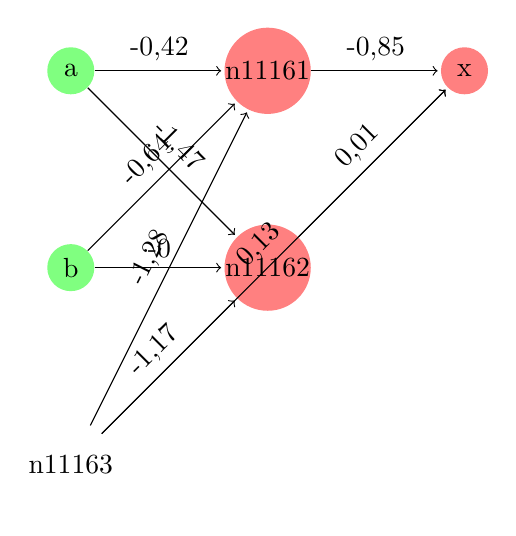
\begin{tikzpicture}[shorten >=1pt,->,draw=black!,node distance=2.5cm]
\tikzstyle{neuron}=[circle,fill=black!25,minimum size=17pt,inner sep=0pt]
\tikzstyle{constant}=[neuron, fill=white!50];
\tikzstyle{sigmoid}=[neuron, fill=red!50];
\tikzstyle{identity}=[neuron, fill=green!50];
\node [identity] (a) {a};
\node [identity,below of=a] (b) {b};
\node [constant,below of=b] (n11163) {n11163};
\node [sigmoid,right of=a] (n11161) {n11161};
\node [sigmoid,below of=n11161] (n11162) {n11162};
\node [sigmoid,right of=n11161] (x) {x};
\path[every node/.style={sloped,anchor=south,auto=false}]
(n11161) edge node {-0,85} (x)
(n11162) edge node {0,01} (x)
(b) edge node {-0} (n11162)
(b) edge node {-0,64} (n11161)
(a) edge node {-1,47} (n11162)
(a) edge node {-0,42} (n11161)
(n11163) edge node {0,13} (x)
(n11163) edge node {-1,17} (n11162)
(n11163) edge node {-1,28} (n11161)
;\end{tikzpicture}
\end{document}